\documentclass[11pt,border=5pt]{standalone}
\usepackage{fontspec}
\setmainfont{cmunrm.otf}[BoldFont=cmunbx.otf,ItalicFont=cmunti.otf,BoldItalicFont=cmunbi.otf]
\usepackage{amsmath}
\usepackage{unicode-math}
\setmathfont{NewCMMath-Regular.otf}
\usepackage{tikz}
\usetikzlibrary{arrows.meta,patterns,angles,quotes}
\begin{document}
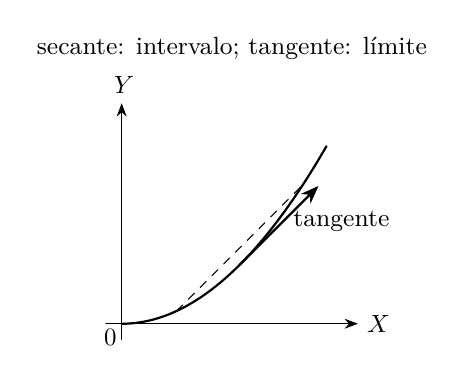
\begin{tikzpicture}[>=Stealth,font=\small,line cap=round,line join=round]
\draw[->,thin] (-0.2,0) -- (3,0) node[pos=1,right] {$X$};
\draw[->,thin] (0,-0.2) -- (0,2.8) node[pos=1,above] {$Y$};
\node at (-0.14,-0.18) {$0$};
\draw[thick] plot coordinates {(0.00000,0.00000) (0.02167,0.00016) (0.04333,0.00063) (0.06500,0.00141) (0.08667,0.00250) (0.10833,0.00391) (0.13000,0.00563) (0.15167,0.00767) (0.17333,0.01001) (0.19500,0.01268) (0.21667,0.01565) (0.23833,0.01893) (0.26000,0.02253) (0.28167,0.02645) (0.30333,0.03067) (0.32500,0.03521) (0.34667,0.04006) (0.36833,0.04522) (0.39000,0.05070) (0.41167,0.05649) (0.43333,0.06259) (0.45500,0.06901) (0.47667,0.07574) (0.49833,0.08278) (0.52000,0.09013) (0.54167,0.09780) (0.56333,0.10578) (0.58500,0.11408) (0.60667,0.12268) (0.62833,0.13160) (0.65000,0.14083) (0.67167,0.15038) (0.69333,0.16024) (0.71500,0.17041) (0.73667,0.18089) (0.75833,0.19169) (0.78000,0.20280) (0.80167,0.21422) (0.82333,0.22596) (0.84500,0.23801) (0.86667,0.25037) (0.88833,0.26305) (0.91000,0.27603) (0.93167,0.28933) (0.95333,0.30295) (0.97500,0.31687) (0.99667,0.33111) (1.01833,0.34567) (1.04000,0.36053) (1.06167,0.37571) (1.08333,0.39120) (1.10500,0.40701) (1.12667,0.42313) (1.14833,0.43956) (1.17000,0.45630) (1.19167,0.47336) (1.21333,0.49073) (1.23500,0.50841) (1.25667,0.52640) (1.27833,0.54471) (1.30000,0.56333) (1.32167,0.58227) (1.34333,0.60151) (1.36500,0.62107) (1.38667,0.64095) (1.40833,0.66113) (1.43000,0.68163) (1.45167,0.70245) (1.47333,0.72357) (1.49500,0.74501) (1.51667,0.76676) (1.53833,0.78882) (1.56000,0.81120) (1.58167,0.83389) (1.60333,0.85689) (1.62500,0.88021) (1.64667,0.90384) (1.66833,0.92778) (1.69000,0.95203) (1.71167,0.97660) (1.73333,1.00148) (1.75500,1.02667) (1.77667,1.05218) (1.79833,1.07800) (1.82000,1.10413) (1.84167,1.13058) (1.86333,1.15734) (1.88500,1.18441) (1.90667,1.21179) (1.92833,1.23949) (1.95000,1.26750) (1.97167,1.29582) (1.99333,1.32446) (2.01500,1.35341) (2.03667,1.38267) (2.05833,1.41225) (2.08000,1.44213) (2.10167,1.47233) (2.12333,1.50285) (2.14500,1.53368) (2.16667,1.56481) (2.18833,1.59627) (2.21000,1.62803) (2.23167,1.66011) (2.25333,1.69250) (2.27500,1.72521) (2.29667,1.75823) (2.31833,1.79156) (2.34000,1.82520) (2.36167,1.85916) (2.38333,1.89343) (2.40500,1.92801) (2.42667,1.96290) (2.44833,1.99811) (2.47000,2.03363) (2.49167,2.06947) (2.51333,2.10561) (2.53500,2.14207) (2.55667,2.17885) (2.57833,2.21593) (2.60000,2.25333)};
\draw[dashed] (0.7,0.1633333333333333) -- (2.3,1.763333333333333);
\draw[->,thick] (1.5,0.75) -- (2.5,1.75) node[pos=0.55,right] {tangente};
\node at (1.4,3.5) {secante: intervalo; tangente: límite};

\end{tikzpicture}
\end{document}
